\documentclass[10pt, biblatex, linguex]{report}
\addbibresource{references.bib}

\pdfauthor{Venkat}
\pdftitle{Analyzing Scalar Implicatures}
%\pdfkeywords{}

\title[PHL394K Term Paper]{How do context and countability modulate\\
                                    scalar implicature strength?}

\author[Venkat]{
                \repauthor{
                    Venkata S Govindarajan \\
                    \institute{University of Texas at Austin} \\
                    \course{phl394k term paper}
                    }
                }

\begin{document}

\maketitle


%\begin{abstract}
%  Scalar Implicatures (SI), such as those from \textit{some} to \textit{not all}, have
%  generally been analysed as a homogenous category of Gricean Conventional
%  Implicatures. However, recent work in psycholinguistics and probabilistic
%  semantics challenges these assumptions, and raises the question -- how does
%  the strength of a scalar implicature interact with its context? In this study,
%  I investigate the dichotomy between scalar implicature strength and its
%  contextual distribution. It has been shown that certain aspects of the
%  linguistic signal (partititves, subjecthood, discourse accesibility) can
%  modulate the strength of the SI -- I wish to investigate whether the countability
%  profiles of nouns have an effect as well.
%\end{abstract}
%
%\begin{keywords}
%scalar implicature, game-theoretic semantics, mass-count nouns
%\end{keywords}

%\blfootnote{$^\dagger${\ttfamily venkatasg@utexas.edu}}

\section{introduction}
\label{sec:introduction}

A core component of the Gricean programme is that language use ought to be
treated as a form of rational activity subject to norms and expectations
\citep{grice_logic_1975}. This
framework has been immensely useful in computing \textit{pragmatic inferences}
where listeners infer information beyond what is the literal meaning
of an utterance. A classical example of this is the scalar implicature:

\ex. \label{ex:1}\a. Mary ate some of the cookies.\label{ex:1a}
                 \b. Mary ate some, but not all, of the cookies.\label{ex:1b}
                 \c. Mary ate all of the cookies.\label{ex:1c}

A speaker who utters \ref{ex:1a} is generally taken to conversationally
implicate \ref{ex:1b}. Most theories treat this inference (and other inferences
that follow from a scale) as a form of generalized \textit{default} inference
that is a consequence of Gricean maxims of Quantity and Quality\citep{grice_logic_1975,
horn_towards_1984}. The speaker
wants to convey as much true information as possible \dash if Mary had eaten all
of the cookies, the speaker would have uttered \ref{ex:1c} instead of
\ref{ex:1a}. The listener in turn, can
reason that since the speaker chose not to utter \ref{ex:1c}, Mary didn't eat
all of the cookies, giving rise to the scalar inference.

This default form of reasoning, while attractive, makes many simplifying
assumptions. Under this reasoning, scalar implicatures are generalized
conversation implicatures (\textbf{GCI}s) that arise because of the presence of
lexicalized items like \textit{some} (rather than special contextual features).
Contextual features of the linguistic signal is
deemed to play a minor role in cancellation of an implicature. This {\rmsc
contextual invariance} assumption follows directly from the {\rmsc homogeneity}
assumption - listeners can either derive the inference or not.


By crowdsourcing human judgements on a corpus, \citet{degen_investigating_2015}
showed that neither assumption holds. She
suggests that the strength of scalar inferences from \textit{some} to
\textit{not all} are highly variable and systematically context-dependent. This
raises interesting implications about the natur and theory behind scalar
implicature. I use her paper as a starting point for this report, and try to
answer two broad questions:

\begin{enumerate}
    \item What is the relationship between the strength of a scalar implicature
          and the \textbf{frequency of its occurence in varying contexts}? This question
          tries to tackle the issue of whether annotators might be biased to
          rate a scalar implicature as stronger if they are more familiar with
          the form of the utterance.
    \item How does the \textbf{countability profile} of \textit{some}-NPs influence
          the strength of the scalar implicature? Similar to how the partitive
          construction is shown to lead to higher implicature strength ratings,
          do count nouns exhibit higher strength ratings than mass nouns?
\end{enumerate}

\S\ref{sec:background} goes over some of the background literature on scalar
implicatures, as well as describing the motivation behind the probabilistic
studies of pragmatic phenomena, including scalar implicatures. In \S\ref{sec:context},
I examine the methodology \citeauthor{degen_investigating_2015} uses to derive
a score for scalar implicature strength, and investigate if this strength is
related to the contextual diversity of the \textit{some}-NPs. Adding to
\possciteauthor{degen_investigating_2015} work showing
how the partitive, determiner strength and discourse accesibility influence
scalar implicature strength, I examine if the countability profile of some-NPs
influence implicature strength in \S\ref{sec:masscount}. I conclude this report
with remarks on my findings and possible future avenues for research
(\S\ref{sec:conclusion})


\section{background}
\label{sec:background}

\subsection{classical theoretic approaches}

Since the focus of this report is on the lexicalized scalar implicature from
\textit{some} to \textit{not all}, let us focus on how this particular scalar
implicature has been studied in literature. Most linguistic theorizing of this
scalar implicatures analyses it as a form of
\textbf{Gricean Conversational Implicature} \citep{grice_logic_1975,
horn_towards_1984, levinson2000presumptive}. This distinguishes them from
Particularized Conversational Implicatures, which as \citet{grice_logic_1975} states,
are carried through because of special features of their context. GCIs on the
other hand, are calculated because of the use of certain forms of words, and
assumptions of rational behavior on the part of the speaker and listener.

A walkthrough of the classical reasoning behind the \textit{some} to \textit{not
all} implicature was illustrated in (\S\ref{sec:introduction}), which
I will not repeat here. Let's focus on the assumptions that this style of
reasoning makes regarding the scalar inference?

\begin{enumerate}
    \item[1] The scalar inference is treated as a \textit{categorical}
             phenomenon. The listener can either derive the inference based on
             the presumption of co-operative behavior and the lexical item
             \textit{some}, or not. There is no room for the listener to
             hold degrees of belief in the scalar inference. This is the
             {\rmsc homogeneity} assumption
    \item[2] The only contextual information that can trigger or act as a cue
             towards the scalar inference is the lexical item \textit{some}
             itself. This is the {\rmsc context independence} assumption.
\end{enumerate}

While there has been acknowledgment of the ability to cancel implicatures
\citep{horn_towards_1984, levinson2000presumptive}, this form of reasoning
doesn't predict that elements of the context play a \textit{systematic} role
towards the generation or cancellation of the scalar implicature.

\subsection{game theoretic approaches}

Recent work in Bayesian pragmatics \citep{frank_predicting_2012,
lassiter_context_2013, rothschild2013game, goodman_pragmatic_2016} have provided
evidence for treating pragmatic phenomena, such as the scalar implicature from
\textit{some} to \textit{not all}, as a form of \textbf{Bayesian probabilistic
reasoning} on the part of speakers and listeners. This framework has been
encapsulated under the heading of \textit{rational speech-act} (RSA) theory.

In the RSA model, a pragmatic listener updates his beliefs about the state of
the world using Bayes' rule, given that the speaker chose an utterance over the
alternatives. The pragmatic speaker in turn is assumed to be approximately
rational and chooses their utterances proportional to their expected utility
(based on how much epistemic utility a \textit{literal} listener would derive
from an utterance). Thus, the pragmatic listener can infer a degree of belief
over the various states of the world conditioned on the speaker's chosen
utterance over the alternatives \citep{goodman_knowledge_2013,goodman_pragmatic_2016}.

How does this affect our understanding of scalar inferences, and what predictions
does it makes? As described by \citeauthor{degen_investigating_2015}, the
revised assumptions and claims are as follows:

\begin{enumerate}
    \item[1] Scalar implicatures are \textbf{probabilistic} rather than
             categorical. The probability reflects the hearer's belief that
             an alternative is more probable than others. This is the strength
             of a scalar implicature.
    \item[2] Scalar implicatures are determined by their context \dash if
             hearers update their beliefs based on their reasoning over
             possible utterances, it stands to reason that \textbf{contextual cues}
             in the linguistic signal would influence their beliefs.
\end{enumerate}

These revised assumptions make a crucial claim \dash scalar implicatures can
now be studied using human judgements over corpora on a continuous scale. This
is the main contribution of \citet{degen_investigating_2015}.

\subsection{strength and contextual variance}

\citet{degen_investigating_2015} performed a corpus and web-based study to
test the two assumptions in the classical model described previously \dash is
the \textit{some} to \textit{not all} scalar implicature {\rmsc homogenous}, and
is it {\rmsc contextually independent}? In her study, participants were asked to
perform a paraphrase similarity task, which she takes as a proxy for the scalar
inference strength. For example, participants were asked to rate the similarity
between the following two statements on a 7-point scale (from not at all similar
to exactly similar):

\ex. \a. Mary ate some of the cookies.
     \b. Mary ate some, but not all, of the cookies.

To investigate the contextual independence assumption, she analyses the effects
of 3 contextual features (or \textit{cues}) on the implicature strength \dash
syntactic partitivity of the \textit{some}-NP, determiner strength, and
discourse accesibility of the \textit{some}-NP. She finds that not only is there
a wide variance in scalar implicature strength contrary to the homogeneity
assumption, this variance in the strength of the scalar implicature is highly
systematic and probabilistically determined by features in the context of the
utterance. Implicature strength is greater on average when \textit{some} occurs
with the partitive, when its usage as a determiner is strong, and when the
\textit{some}-NP is relatively discourse accessible.

Using her dataset and models as a starting point, I will start by investigating
the relationship between implicature strength and the \textbf{contextual
diversity} of the \textit{some}-NP.

\section{contextual diversity and strength}
\label{sec:context}

\posscitet{degen_investigating_2015} annotation protocol asked annotators to
rate the similarity between a \textit{some} utterance with a paraphrase
that substituted \textit{some} with \textit{some but not all}, like in
\ref{ex:paraphrase}. If two statements are judged to be highly similar (on the
7-point Likert scale), she concludes that the scalar implicature is encoded
strongly in the \textit{some} utterance.

\ex.\label{ex:paraphrase} \a. I like, I like to read \textit{some} of the philosophy stuff.
     \b. I like, I like to read \textit{some, but not all}, of the philosophy stuff.

This paraphrase task is a novel measurement of scalar implicature strength,
and \citeauthor{degen_investigating_2015} discussed how certain effects of
context(monotonicity), shifts in Question Under Discussion, and annotator
variability could affect its interpretability. However, this raises the question
\dash if an annotator
says that the \textit{some} utterance and its \textit{some, but not all}
paraphrase are highly similar (or dissimilar), does that mean that the scalar
implicature is necessarily strong (or weak)? For example, might annotators choose
to rate two statements as dissimilar because of their unfamiliarity with the
\textit{some}-NP and its usage in a \textit{some, but not all} construction?
Narrowing down the
question to one of \textbf{contextual diversity}, does a \textit{some} to
\textit{some, but not all} scalar implicature need to occur in a wide variety
of contexts to be considered a strong implicature?


\paragraph{Data Analysis} To investigate whether the contextual diversity of the
object of a \textit{some-not all} implicature modulates its strength, I performed
a simple analysis of the \textit{some}-NPs from \citet{degen_investigating_2015}.
The \textit{some}-NPs were extracted from the dependency parse of each sentence
\citep{qi2020stanza} by finding those NPs that were immediately governed by (or
that governed) \textit{some} \citep{white-EtAl:2016:EMNLP2016,
zhang-EtAl:2017:IWCS}. To simplify the analysis, only one-word NPs were chosen
for further analysis. Each NP was lemmatized, and the frequency of occurence of
the lemma in the corpus was calculated. In total, \textbf{509} unique lemmas
were found in \textbf{1291} unique sentences. The frequency of a lemma is defined
as the number of unique sentences which contain the lemma in question in our
corpus. I take this to be a proxy for the \textbf{contextual diversity} of a
lemma.

\begin{figure}[t]
    \centering
    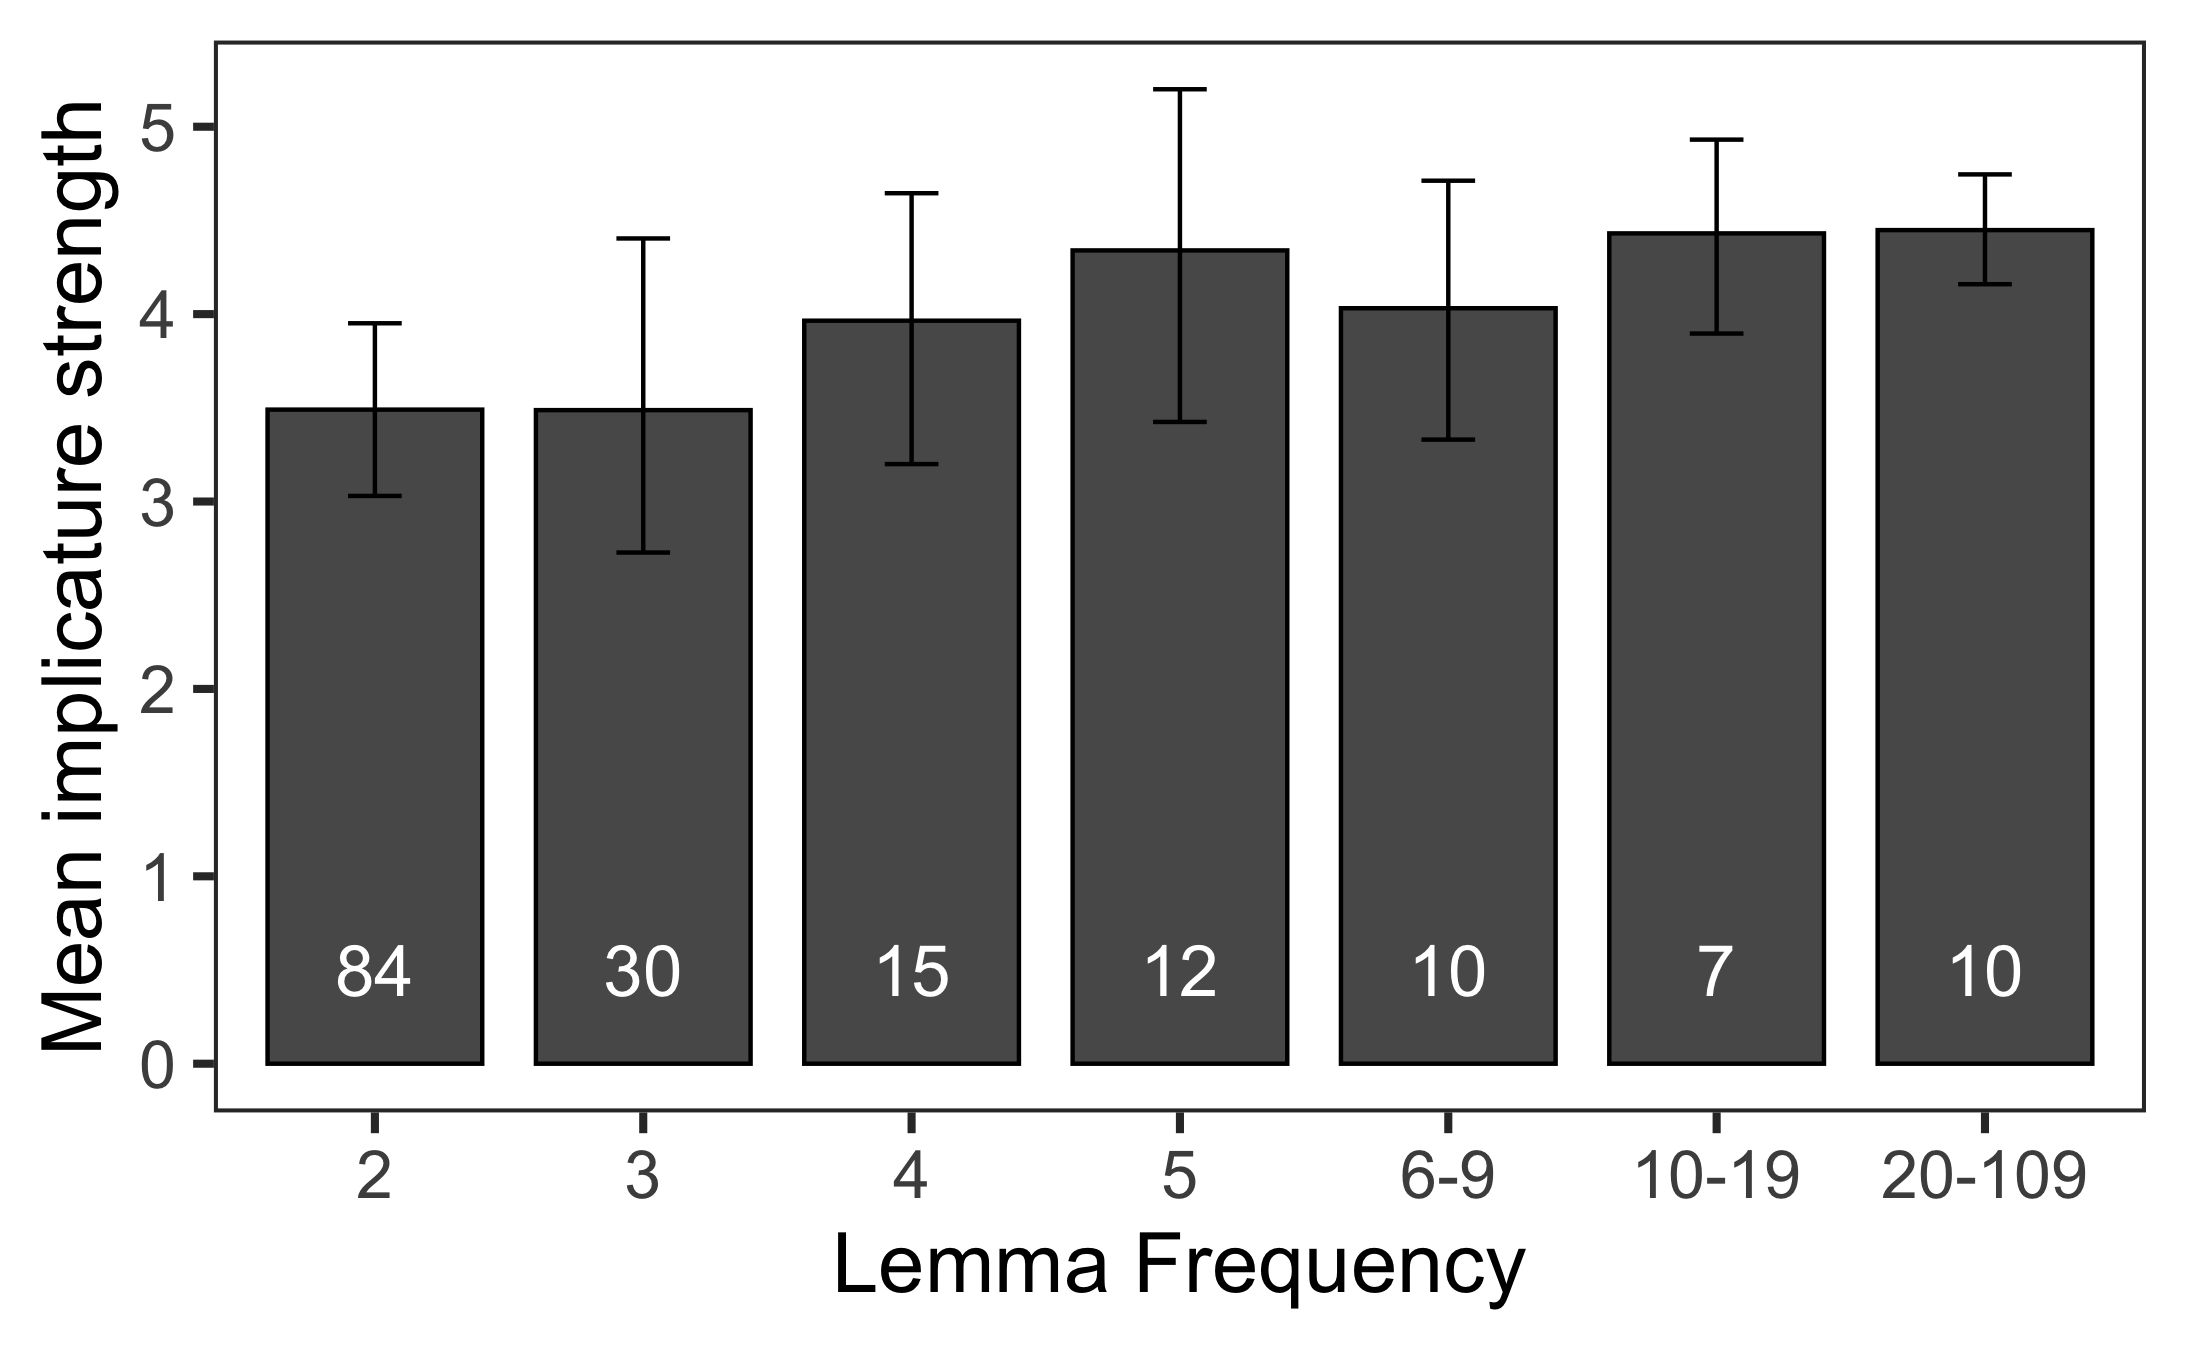
\includegraphics[width=\linewidth]{images/lemma.png}
    \caption{Mean implicature strength versus lemma frequency. The numbers inside
             each bar indicate the number of unique lemmas.}
    \label{fig:lemma}
\end{figure}

\begin{figure}[t]
    \centering
    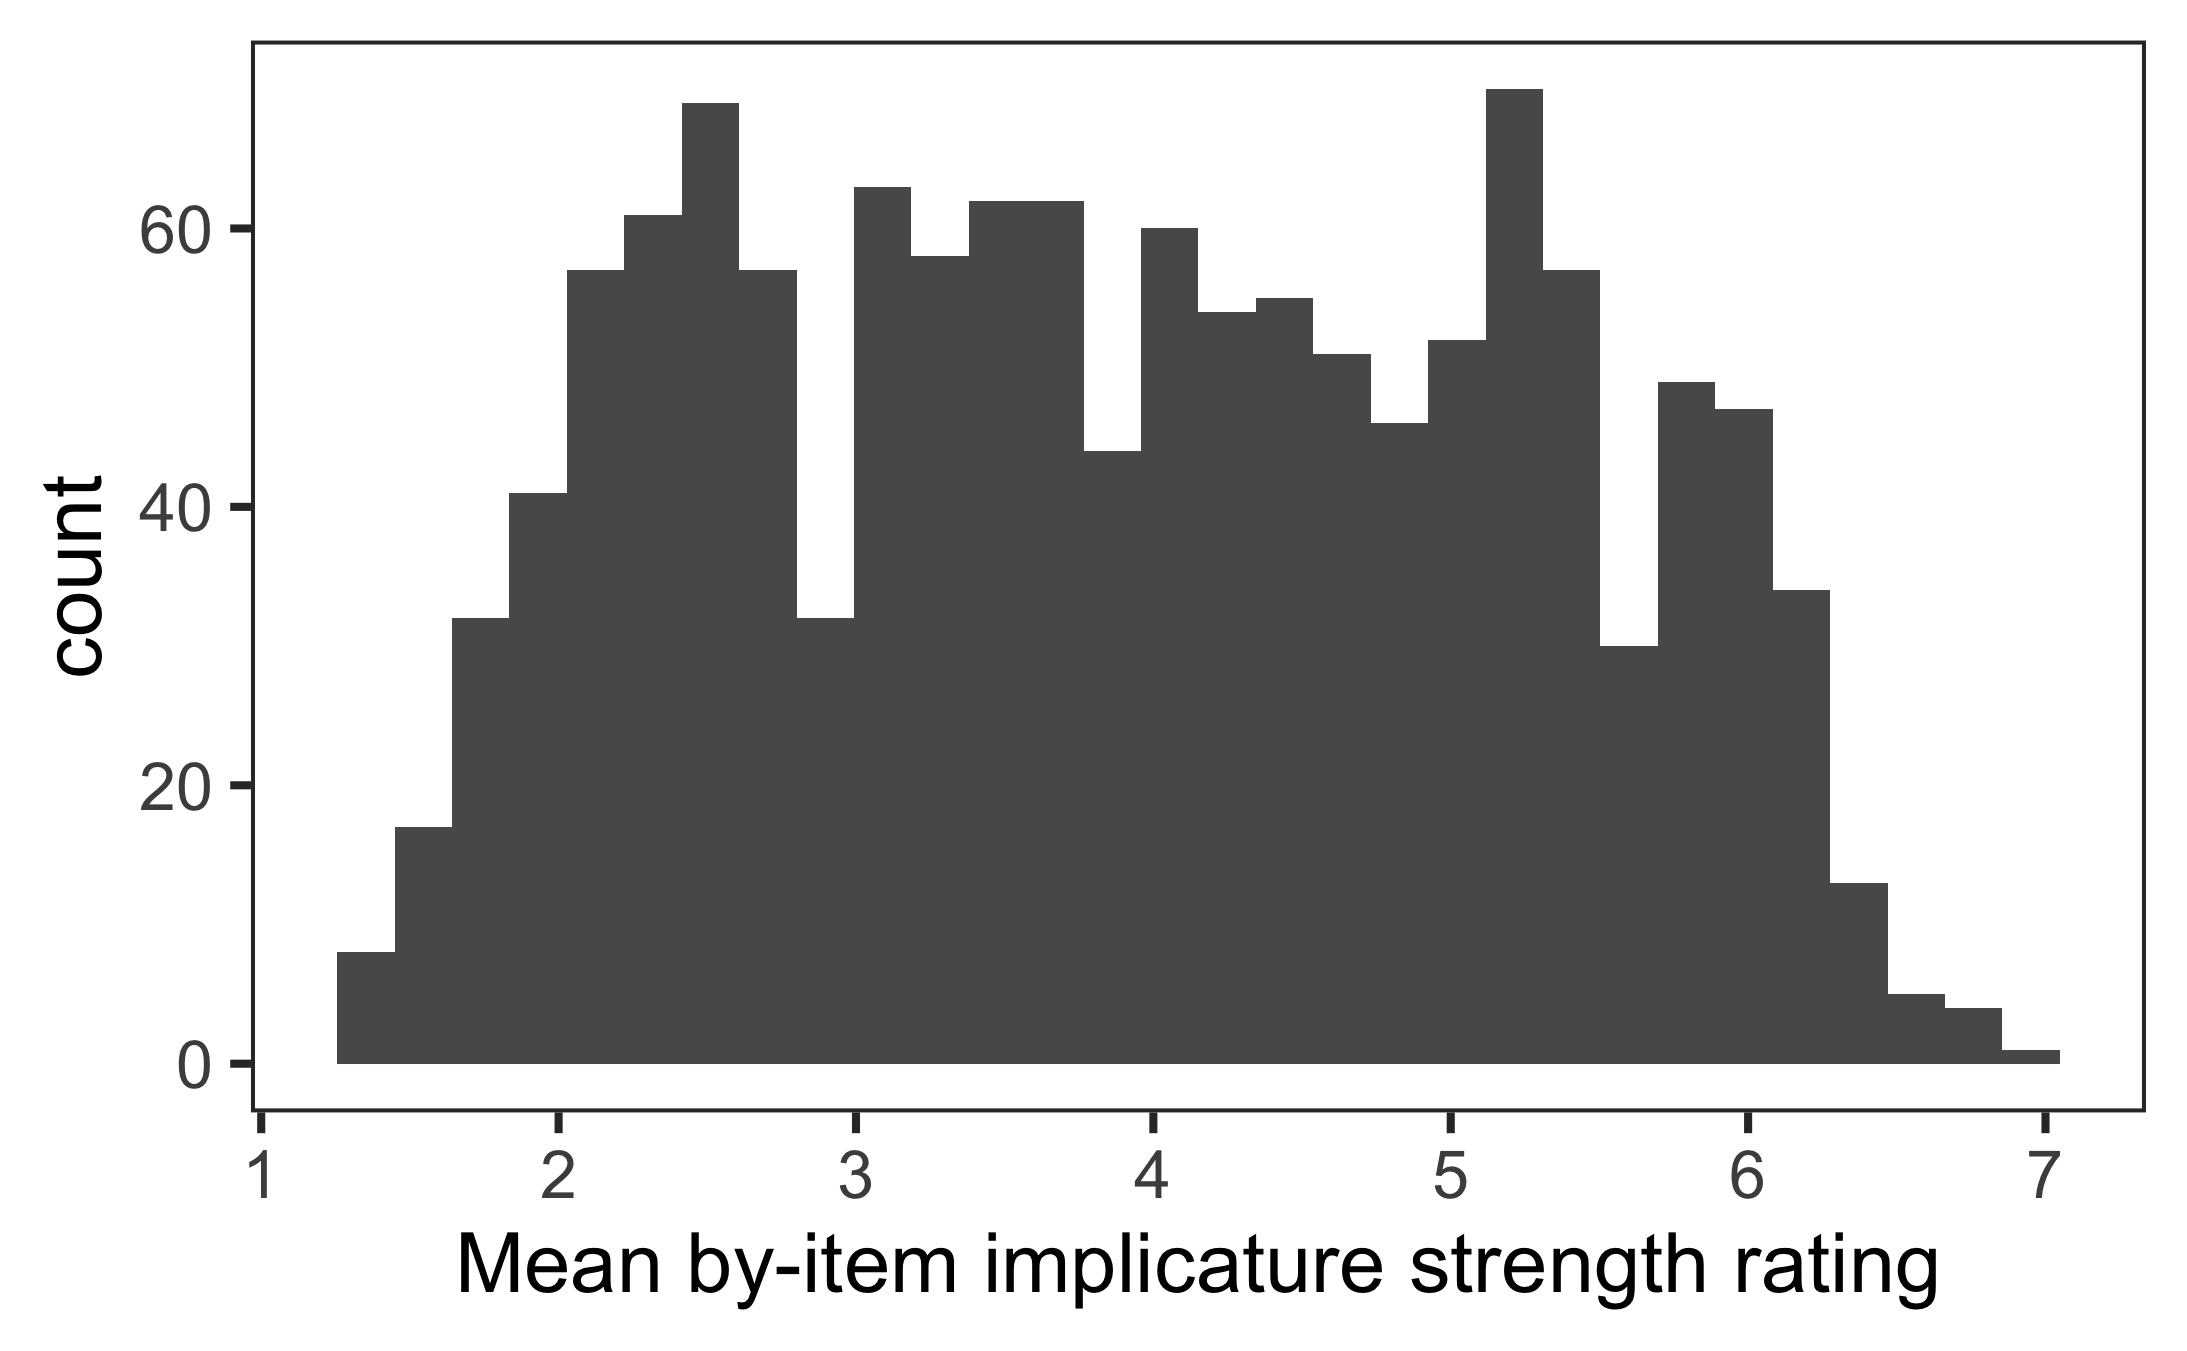
\includegraphics[width=\linewidth]{images/dist.png}
    \caption{Average by-item implicature strength ratings in our restricted dataset.}
    \label{fig:dist}
\end{figure}


\paragraph{Results} Each sentence was rated by 10 different annotators in the
dataset \dash all results henceforth report the average implicature strength
assigned by all annotators. Figure \ref{fig:lemma} shows the average implicature
strength rating against the lemma frequency (the number inside each bar indicates
how many unique lemmas had that frequency \dash for example 15 unique lemmas
occured in 4 different sentences and had an average implicature strength of
around 4). While there is a disparity in distribution of the lemmas which is to be
expected (highly frequent lemmas occur are fewer), we also notice that there is
a slight tendency for highly frequent lemmas to have a higher mean
implicature strength.

For an objective measure for whether lemma frequency is correlated with implicature
strength, we use the Spearman Rank correlation test. A non-parametric test was
chosen since Figure \ref{fig:dist} shows that the mean by-item implicature strength
distribution is not normal, and a Shaprio-Wilk's test \citep{shapiro_analysis_1965}
verifies this observation(\textit{W}=0.96, \textit{p}<2.2e-16). The Spearman's
correlation coefficient between lemma frequency and implicature strength ($\rho$)
is 0.51 (\textit{S}=651, \textit{p}<0.05). The Pearson's correlation coefficient
was  also calculated, and found to be 0.44 (\textit{t}=2.09, df=18,
\textit{p}=0.051).

\paragraph{Discussion} We started with the question of whether paraphrase
similarity was a reliable indicator of scalar implicature strength, or whether
external factors might influence the similarity rating \textbf{independent} of the
scalar implicature strength. I chose to investigate one facet of this
interaction \dash Is the implicature strength of the lemma of the
\textit{some}-NP correlated with its frequency of occurence in unique contexts?
The results above show that a significant correlation does exist.
\textbf{Highly frequent lemmas are correlated with a higher implicature strength
rating}. For example, given below are sentences which have the 2 most frequent
lemmas (\textit{people} and \textit{thing}) along with their mean implicature
raing and their corresponding paraphrase:

\ex. \a. I mean, \textbf{some people} sing, \hfill \textbf{5.5}
     \b. I mean, \textbf{some, but not all}, people sing,

\ex. \a. i, i'm glad, to see \textbf{some of these things}, i think .\hfill \textbf{4.7}
     \b. i, i'm glad, to see\textbf{ some, but not all of these} things, i think .

Now consider some ratings for the lemmas \textit{noise} whose frequency was 2,
and \textit{information}, whose frequency was 7:

\ex. \a. and i was picking up, uh, \textbf{some background noise},.\hfill \textbf{2.1}
     \b.?and i was picking up, uh, \textbf{some, but not all, background noise}.\label{ex:unacc-a}

\ex. \a. i got \textbf{some interesting information} about crawfish \hfill \textbf{2.5}
     \b. ?i got \textbf{some, but not all, interesting information} about crawfish\label{ex:unacc-b}

One potential reason for less frequent lemmas
having lower implicature strength ratings could be that the paraphrases tend to be
more \textbf{unacceptable} like in \ref{ex:unacc-a} and \ref{ex:unacc-b}. While it might
appear that these unacceptable sentences are more likely to occur with
low-strength determiner uses of \textit{some}, determiner
strength by itself wasn't found to be indicative of the unacceptability of
certain statements (as discussed in \S 2.3.2 of \citet{degen_investigating_2015}
), and there isn't a significant correlation between lemma frequency and
determiner strength either ($\rho$=-0.35, \textit{p}=0.134).

It might be tempting to attribute the lower ratings for less frequent lemmas to
annotators being more likely to give high ratings towards lemmas
they are more familiar with. However, the
lemma frequencies used here are not indicative of real-word distributions, or the
entire range of contexts in which they may occur. For instance, the lemma
\textit{music} occurs only twice in the dataset, and yet has high
implicature strength ratings:

\ex. e-, even in some families some people talk a little bit different. \hfill \textbf{5.3}

Further analysis would be necessary to verify if the observed correlation is
merely an artifact of the datset under study, or indicative of a possible
factor to consider when deriving scalar implicature strength based on a
similarity score.

\section{mass-count distinction}
\label{sec:masscount}

As already discussed, \citet{degen_investigating_2015} found that the
partitive, determiner strength, and discourse accessibility provide reliable cues
for scalar implicature strength. In this section, I wish to investigate if the
\textbf{countability} profile of \textit{some}-NPs are also a significant
contextual cue in determining scalar implicature strength.

The classical mass-count distinction is a morphosyntactic distinction that is
generally taken to have semantic significance \citep{moltmann2020}. Mass nouns
(such as rice, wood and water) are generally found to differ from count nouns
(like apples, chairs and carpets) in several syntactic and and semantic
dimensions. For instance mass nouns generally lack a plural(\textit{*I ate rices}),
cannot take cardinal or ordinal numerals(\textit{*two waters}), and also disallow
singular quantifiers (\textit{*every water}). The semantics of mass and count nouns
are also different, although there are differing views on how to interpret the
distinction between the two \citep{moltmann1998part,moltmann1998part,
link2002logical,champollion2016mereology,champollion2017parts,krifka1989nominal,
moltmann2020}.

Recent work has questioned the assumption underlying the countable - noncountable
contrast \citep{grimm2020, grimmgrammatical2018} \dash is it ontologically based
or is there a scale of countability between prototypically countable nouns and
non-countable (mass) nouns? These questions are relevant for studying scalar
implicatures in light of the varying semantics of mass nouns:

\ex. \a. I ate some rice for lunch.\label{ex:mass-a}
     \b. ?I ate some, but not all, rice for lunch.\label{ex:mass-b}

\ref{ex:mass-a} is not similar in meaning to \ref{ex:mass-b}. Moreover,
\ref{ex:mass-b} as a sentence is, if not ungrammatical, possibly unacceptable
(there is, however, a possible reading where the speaker is saying that they
didn't eat \textit{only} rice for lunch. I ignore this reading). The incongruity
of the \textit{some but not all} utterance disappears when the
partitive is used:

\ex. \a. I ate some of the rice for lunch.\label{ex:mass-p-a}
     \b. I ate some, but not all, of the rice for lunch. \label{ex:mass-p-b}

This brings up an interesting question \dash could the lower
implicature strength ratings with sentences that have low strength determiners or
non-partitive clauses be explained by the countability profile of their
\textit{some}-NPs? Thus, the questions I wish to ask are as follows:

\begin{enumerate}
    \item[1] Does the countability profile of the object NP under \textit{some}
          have an impact on the implicature strength ratings?
    \item[2] If it does, is it wholly independent from the effects of determiner strength and
          partitivity?
\end{enumerate}


\paragraph{Data Analysis} Similar to the context analysis in \S \ref{sec:context},
the relevant NP lemmas were extracted from the dependency parse of sentences in
the dataset. Once again, this analysis is restricted to one word NPs. The
{\rmsc celex} database \citep{celex2} is a lexical database of English that
uses a classical countability classification \dash countable, uncountable or both.
Using this classification method, we add two cues
corresponding to each lemma in the dataset \dash {\rmsc mass} and
{\rmsc count}, each of which has either the values \textit{yes} or \textit{no}.
{\rmsc count} and {\rmsc mass} are treated separately as there are some lemmas
that can function as mass or count depending on the context and their word sense,
and because mass and count nouns are known to undergo shifts to their counterparts
in taxonomic and packaged readings \citep{moltmann2020}. Sentences for which the
lemmas were not found in the {\rmsc celex} database were discarded, thus providing us
with \textbf{1133 sentences} to perform further analysis on.

To verify if {\rmsc mass} and {\rmsc count} are reliable cues that influence the
scalar implicature strength determined by annotators, I report the results of
the same linear mixed effects regression models \citep{baayen2008mixed} used in
\citet{degen_investigating_2015}, with the new countability columns included as
fixed effects in the regression. To recap, the mixed-effects linear regression
model predicts the implicature strength from fixed effects of interest (the cues
under investigation) along with random by-item intercepts, random by-participant
intercepts, and random by-participant slopes for all fixed effects. {\rmsc mass}
and {\rmsc count} were added as fixed effects (and allowed to interact with the
{\rmsc partitive} and {\rmsc determiner} fixed effects), and random by-participant
slopes were added for each as well. Three types of models were considered \dash
the basic model only considered random effects, the intermediate model only
considered fixed effects, while the final model considered both fixed and
random effects. The final model from \citet{degen_investigating_2015} was used
as a baseline for comparing the impact of adding {\rmsc count} and {\rmsc mass}
as fixed effects and random by-participant effects.

\begin{figure}[t]
    \centering
    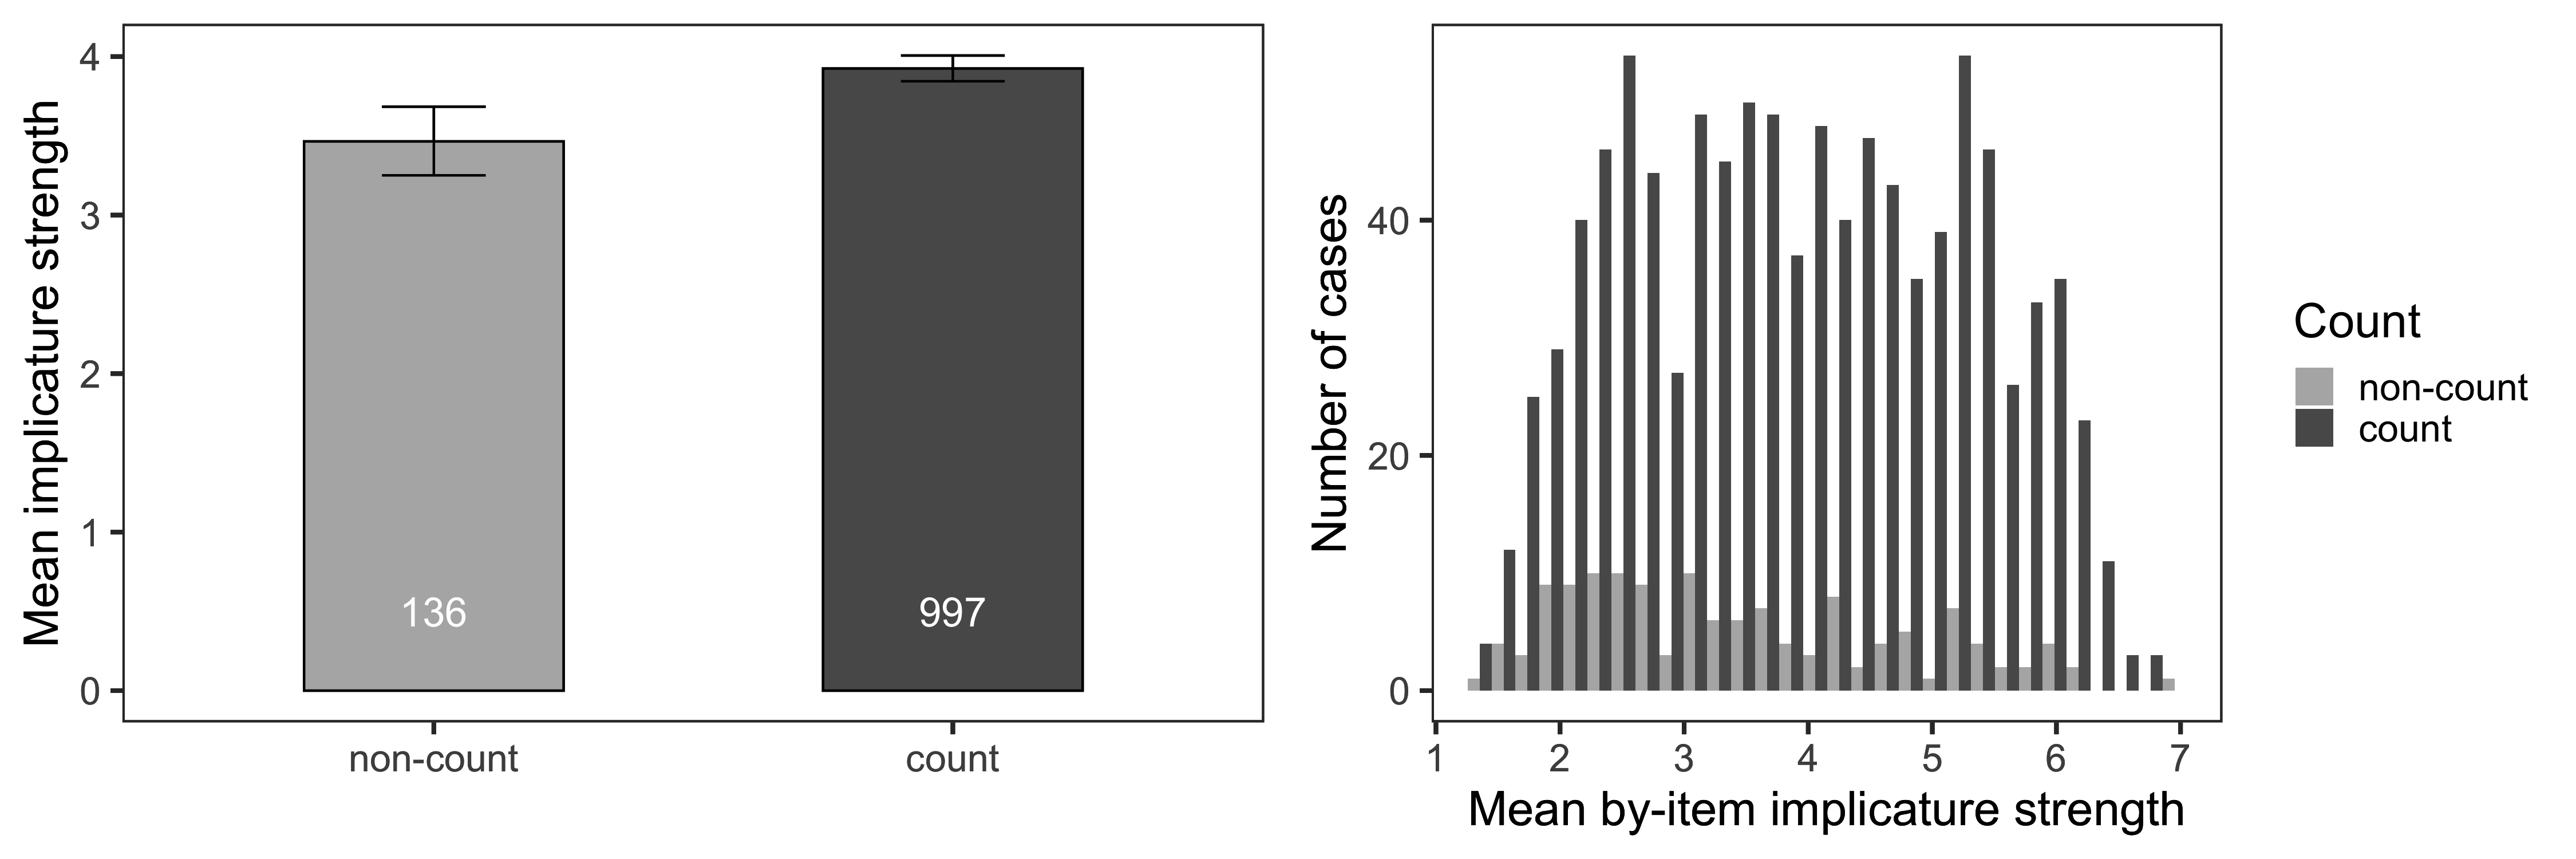
\includegraphics[width=\linewidth]{images/count.png}
    \caption{Mean implicature strength ratings (left) and distribution of mean
             by-item ratings (right) for non-count and count some-NPs.}
    \label{fig:count}
\end{figure}

\begin{figure}[t]
    \centering
    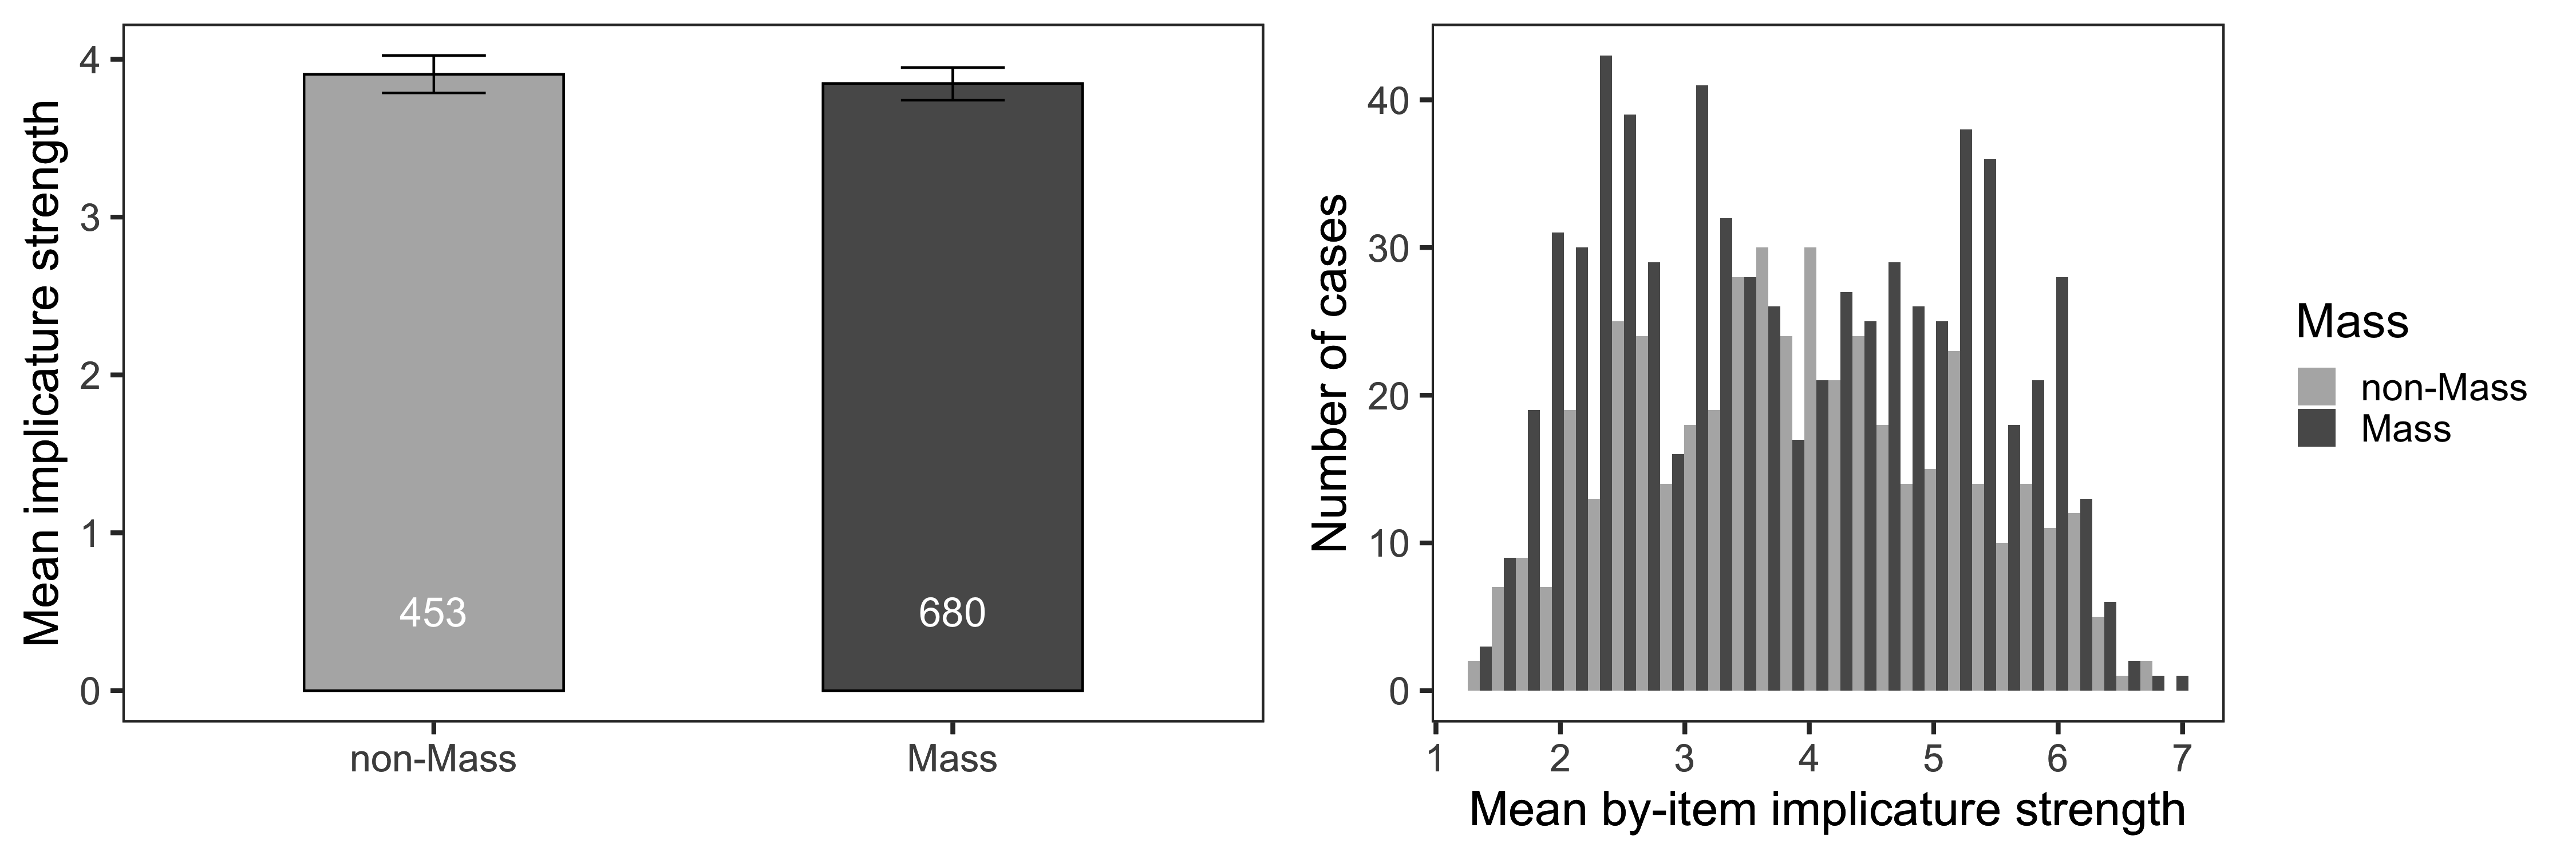
\includegraphics[width=\linewidth]{images/mass.png}
    \caption{Mean implicature strength ratings (left) and distribution of mean
             by-item ratings (right) for non-mass and mass some-NPs.}
    \label{fig:mass}
\end{figure}


\paragraph{Results} \textit{count} items have
an average strength rating of 3.46, and they are higher than \textit{non-count}
items which have an average rating of 3.92 (Figure \ref{fig:count}). Similarly,
\textit{non-mass} items (which could be considered analogous to count items) have
a slightly higher average implicature strength rating (3.90) than \textit{mass}
items (3.85) (Figure \ref{fig:mass}). However, to conclude that either {\rmsc mass} or {\rmsc count} are
reliable cues for scalar implicature strength, we need to turn to the performance
and coefficients of our linear mixed-effects model.

\begin{table}[t]
    \centering
    \begin{tabular}{lrrr}
         & Basic Model & Intermediate Model & Final Model  \\ \midrule
        Degen 2015 & 0.099 & 0.264 & 0.457 \\
        Degen 2015+Mass+Count & 0.099 & 0.271 & 0.461 \\
    \end{tabular}
    \caption{Proportion of variance (Conditional R$^2$) explained by each model.}
    \label{tab:models}
\end{table}

Table \ref{tab:models}
reports the conditional R$^2$ of various models on our restricted dataset. The
conditional R$^2$ measures the percentage of variance explained by the fixed and
random effects of our model. We observe that while the {\rmsc mass} and {\rmsc
count} fixed effects do help in boosting the performance of our model, the
improvement is very small. This could mean that the mass-count distinction does
not play a major role in determining scalar implicature strength. However this
could also be an indication that our method for incorporating the countability
profile of NPs for analysis needs to be improved. The model coefficients for the
{\rmsc mass} and {\rmsc count} factors in Table \ref{tab:coeffs} indicate that
the cues as incorporated currently do not add any relevant information towards
determining implicature strength. The slopes of the individual fixed effects are
small and insignificant (as suggested by the p-values). While there does seem to
be some interaction between our new fixed effects with the previous ones, none
of them are potentially significant.


\begin{table}[t]
    \centering
    \begin{tabular}{lrrrl}
    \multicolumn{1}{l}{}&\multicolumn{1}{c}{Coef $\beta$}&\multicolumn{1}{c}{SE($\beta$)}&
    \multicolumn{1}{c}{\textbf{t}}&\multicolumn{1}{c}{$p$}\tabularnewline
    \midrule
    Intercept&$ 3.94$&$0.06$&$63.2$&\textbf{\textless .0001}\tabularnewline
    Partitive&$ 0.90$&$0.12$&$ 7.4$&\textbf{\textless .0001}\tabularnewline
    Strength&$-0.53$&$0.06$&$-9.1$&\textbf{\textless .0001}\tabularnewline
    Mass&$ 0.09$&$0.08$&$ 1.2$&\textgreater 0.25\tabularnewline
    Count&$ 0.08$&$0.14$&$ 0.6$&\textgreater 0.55\tabularnewline
    %Linguistic mention&$ 0.29$&$0.07$&$ 4.1$&\textbf{\textless .0001}\tabularnewline
    %Subjecthood&$ 0.37$&$0.11$&$ 3.4$&\textbf{\textless .001}\tabularnewline
    %Modification&$ 0.17$&$0.07$&$ 2.5$&\textbf{\textless .05}\tabularnewline
    %Sentence length&$ 0.19$&$0.05$&$ 3.6$&\textbf{\textless .001}\tabularnewline
    %Partitive:Strength&$ 0.24$&$0.11$&$ 2.3$&\textbf{\textless .05}\tabularnewline
    Partitive:Mass&$ 0.19$&$0.20$&$ 1.0$&\textgreater 0.33\tabularnewline
    Strength:Mass&$-0.14$&$0.10$&$-1.5$&\textgreater 0.15\tabularnewline
    Partitive:Count&$-0.50$&$0.44$&$-1.1$&\textgreater 0.26\tabularnewline
    Strength:Count&$ 0.16$&$0.18$&$ 0.9$&\textgreater 0.35\tabularnewline
    Mass:Count&$ 0.49$&$0.28$&$ 1.8$&\textgreater 0.08\tabularnewline
    %Linguistic mention:Subjecthood&$ 0.26$&$0.22$&$ 1.2$&\textgreater 0.24\tabularnewline
    %Linguistic mention:Modification&$ 0.34$&$0.14$&$ 2.5$&\textbf{\textless .05}\tabularnewline
    %Subjecthood:Modification&$ 0.25$&$0.19$&$ 1.3$&\textgreater 0.19\tabularnewline
    %Partitive:Strength:Mass&$ 0.38$&$0.21$&$ 1.8$&\textgreater 0.07\tabularnewline
    %Partitive:Strength:Count&$-0.69$&$0.42$&$-1.7$&\textgreater 0.1\tabularnewline
    %Partitive:Mass:Count&$-1.11$&$0.81$&$-1.4$&\textgreater 0.17\tabularnewline
    %Strength:Mass:Count&$-0.65$&$0.37$&$-1.7$&\textgreater 0.08\tabularnewline
    %Linguistic mention:Subjecthood:Modification&$ 0.55$&$0.45$&$ 1.2$&\textgreater 0.22\tabularnewline
    %Partitive:Strength:Mass:Count&$ 0.82$&$0.78$&$ 1.1$&\textgreater 0.29\tabularnewline
    \end{tabular}
    \caption{Model coefficients for our final model with {\rmsc mass} and {\rmsc
             count} added as fixed effects}
    \label{tab:coeffs}
\end{table}

\paragraph{Discussion} Incorporating {\rmsc mass} and {\rmsc count} as factors
from the {\rmsc celex} database did not help in improving the performance of
our model significantly, nor do they seem to be reliable cues towards
scalar implicature strength one way or another. While I had hypothesized that
one reason could be that the partitive or determiner strength could interact
with the countability profile of NPs under \textit{some}, our model coefficients
show this not to be the case.

Future work needs to look into whether expanding the definition of countability
to include more information from {\rmsc celex}, such as \textit{singularia
tantum}, which is encoded separately from \textit{uncountable} nouns in the
database (presumably to distinguish between uncountable nouns that do have a
plural form versus those that don't). In addition, \textit{pluralia tantum}
information from the database needs to be incorporated as well. These lemmas
are the most interesting for further study since they don't fall neatly into
classical countability categories. Consider the
following examples from the dataset of \textit{pluralia tantum} NPs:

\ex. \a. and then with that i try and handle, you know, \textbf{some of the
         clothes} that the girls need and things like that,\hfill \textbf{4.4}
     \b. i got \textbf{some interesting information} about crawfish \hfill \textbf{2.5}
     \b. uh, she can't eat \textbf{some cream cheese}. \hfill \textbf{3.2}
     \b. i like \textbf{some country music}.\hfill \textbf{6.9}

The \textit{tantum} NPs in the examples above showcase a wide range of implicature
strengths. Future work needs to look into whether incorporating countability
profile of NPs as a real-valued score between prototypical count NPs, and
prototypical mass NPs provide more reliable cues towards the scalar implicature
\citep{grimmgrammatical2018}.

\section{conclusion}
\label{sec:conclusion}

This report adds to the growing body of work showing that probabilistic models
and theories of scalar implicatures (and other pragmatic phenomena) are fruitful
areas of research which translate well to human judgement and statistical
studies. I have tried to answer two major questions \dash is the measure
of scalar implicature strength related to the contextual diversity of the
\textit{some}-NP, and does the countability profile of the \textit{some}-NP
provide a reliable cue towards scalar implicature strength?

A significant positive correlation was found between the frequency of the
\textit{some}-lemma in the dataset and its implicature strength.One plausible
explanation for the lower ratings of less frequent lemmas in the
dataset is the general unacceptability/weirdness of the paraphrase, which may
cue annotators to rate them as less similar. Future work can look into whether
the addition of an additional question where annotators are asked if the
paraphrase is ungrammatical and/or unacceptable influences their similarity
ratings \citep{white_computational_2016}.

No significant interaction was found between the countability profile of
\textit{some}-NPs and implicature strength. The lack of a reliable effect
suggests that future work needs to look into better
methods of calculating and incorporating countability profiles into a
probabilistic model of scalar implicatures.

\begin{addresses}
  \begin{address}
    Venkata S Govindarajan \\
    Department of Linguistics \\
    University of Texas at Austin \\
    \email{venkatasg@utexas.edu}
  \end{address}
\end{addresses}


\newpage

% References
\pagestyle{empty}
\printbibliography[title={references}]

\end{document}
